\documentclass[12pt]{article}
\usepackage[utf8]{inputenc}
\usepackage[spanish,es-lcroman, es-tabla]{babel}
\usepackage[autostyle,spanish=mexican]{csquotes}
\usepackage{amsmath}
\usepackage{amssymb}
\usepackage{nccmath}
\numberwithin{equation}{section}
\usepackage{amsthm}
\usepackage{graphicx}
\usepackage{epstopdf}
\DeclareGraphicsExtensions{.pdf,.png,.jpg,.eps}
\usepackage{color}
\usepackage{float}
\usepackage{multicol}
\usepackage{enumerate}
\usepackage[shortlabels]{enumitem}
\usepackage{anyfontsize}
\usepackage{anysize}
\usepackage{array}
\usepackage{multirow}
\usepackage{enumitem}
\usepackage{cancel}
\usepackage{tikz}
\usepackage{circuitikz}
\usepackage{tikz-3dplot}
\usetikzlibrary{babel}
\usetikzlibrary{shapes}
\usepackage{bm}
\usepackage{mathtools}
\usepackage{esvect}
\usepackage{hyperref}
\usepackage{relsize}
\usepackage{siunitx}
\usepackage{physics}
%\usepackage{biblatex}
\usepackage{standalone}
\usepackage{mathrsfs}
\usepackage{bigints}
\usepackage{bookmark}
\spanishdecimal{.}

\setlist[enumerate]{itemsep=0mm}

\renewcommand{\baselinestretch}{1.5}

\let\oldbibliography\thebibliography

\renewcommand{\thebibliography}[1]{\oldbibliography{#1}

\setlength{\itemsep}{0pt}}
%\marginsize{1.5cm}{1.5cm}{2cm}{2cm}


\newtheorem{defi}{{\it Definición}}[section]
\newtheorem{teo}{{\it Teorema}}[section]
\newtheorem{ejemplo}{{\it Ejemplo}}[section]
\newtheorem{propiedad}{{\it Propiedad}}[section]
\newtheorem{lema}{{\it Lema}}[section]

\newcommand{\sech}{\mathrm{sech} \,}
\usepackage{tikz-3dplot}
%\author{M. en C. Gustavo Contreras Mayén. \texttt{curso.fisica.comp@gmail.com}}
\title{Sistemas Coordenados Curvilíneos Generalizados \\ {\large Matemáticas Avanzadas de la Física}}
\date{ }
\begin{document}
%\renewcommand\theenumii{\arabic{theenumii.enumii}}
\renewcommand\labelenumii{\theenumi.{\arabic{enumii}}}
\maketitle
\fontsize{14}{14}\selectfont
\section{Sistemas coordenados cilíndricos $(q_{1}, q_{2}, z)$}
En esta sección trataremos con una clase especial de sistemas de coordenadas curvilíneas definidas por las ecuaciones
\begin{equation}
x = x(q_{1}, q_{2}), \hspace{0.5cm} y = y(q_{1}, q_{2}), \hspace{0.5cm} z = q_{3}
\label{eq:ecuacion_A_08_01}
\end{equation}
Como $q_{1}$ y $q_{2}$ dependen solo de $x$ e $y$, pueden considerarse como coordenadas curvilíneas en un \emph{plano} perpendicular al eje z.

Las curvas en este plano en las que $q_{1}$ y $q_{2}$ son constantes, son entonces los generadores de las superficies de coordenadas $q_{1} = \mbox{ constante}$ y $q_{2} = \mbox{ constante}$, obtenidas moviendo el plano perpendicularmente a sí mismo. Estas superficies coordinadas tienen la forma de cilindros. 
\subsection{Coordenadas cilíndricas circulares $(\rho, \varphi, z)$}.
Las coordenadas cilíndricas circulares
\begin{equation}
    q_{1} = \rho, \hspace{0.5cm} q_{2} = \varphi, \hspace{0.5cm} q_{3} = z
    \label{eq:ecuacion_A_09_01}
\end{equation}
están definidas por las relaciones
\begin{equation}
    x = \rho \: \cos \varphi, \hspace{0.5cm} y = \rho \: \sin \varphi, \hspace{0.5cm} z = z
    \label{eq:ecuacion_A_09_02}
\end{equation}
Que pueden resolverse explícitamente para las coordenadas curvilíneas
\begin{equation}
    \rho = (x^{2} + y^{2})^{1/2}, \hspace{0.5cm} \varphi = \tan^{-1} \left( \dfrac{y}{x} \right), \hspace{0.5cm} z =z
    \label{eq:ecuacion_A_09_03}
\end{equation}
\begin{figure}
    \centering
    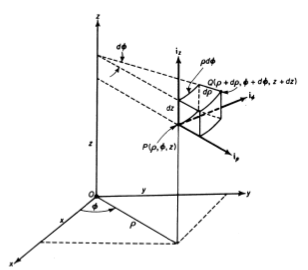
\includegraphics{./Imagenes/Sistema_01_Cilindrico_Circulares.png}
    \caption{Coordenadas cilíndricas circulares.}
\end{figure}
\subsection{Sistemas de coordenadas cilíndricas conjugadas.}
Transformaciones del tipo
\begin{equation}
    x + i \: y = f (q_{1} + i \: q_{2}), \hspace{0.5cm} z = q_{3}
    \label{eq:ecuacion_A_10_01}
\end{equation}
generan sistemas de coordenadas curvilíneas cilíndricas, al igualar las partes real e imaginaria, se obtiene
\begin{equation*}
    x = x(q_{1}, q_{2}), \hspace{0.5cm} y = y(q_{1}, q_{2}), \hspace{0.5cm} z = q_{3}
\end{equation*}
Aplicando las ecuaciones de Cauchy-Riemann a las ecs. (\ref{eq:ecuacion_A_10_01}), se tienen
\begin{equation}
    \dfrac{\partial x}{\partial q_{1}} = \dfrac{\partial y}{\partial q_{2}}, \hspace{0.5cm} \dfrac{\partial x}{\partial q_{2}} = - \dfrac{\partial y}{\partial q_{1}}
    \label{eq:ecuacion_A_10_02}
\end{equation}
Esto sería prueba suficiente para demostrar que el sistema de coordenadas curvilíneo generado por la ec. (\ref{eq:ecuacion_A_10_01}), $(q_{1}, q_{2}, q_{3})$ -en ese orden-, forman un sistema de coordenadas ortogonal y derecho, cuyos factores de escala están dados por:
\begin{equation}
    \dfrac{1}{h_{1}^{2}} = \dfrac{1}{h_{2}^{2}} = \left( \dfrac{\partial x}{\partial q_{1}} \right)^{2} + \left( \dfrac{\partial y}{\partial q_{1}} \right)^{2} =  \ldots = \left| \dfrac{d (x + i \: y)}{d (q_{1} + i \: q_{2})} \right|^{2}
    \label{eq:ecuacion_A_10_03}  
\end{equation}
y para el último factor
\begin{equation}
    h_{3} = 1
    \label{eq:ecuacion_A_10_4}
\end{equation}
\subsection{Coordenadas elípticas cilíndricas $(\xi, \eta, z)$.}
La transformación
\begin{equation}
    x + i \: y = c \: \cosh (\xi + i \: \eta)
    \label{eq:ecuacion_A_11_01}
\end{equation}
con $c > 0$, cede, al expandir el lado derecho e igualar partes reales e imaginarias en
\begin{equation}
    x = c \: \cosh \xi \: \cos \eta, \hspace{0.5cm} y = c \: \sinh \xi \: \sin \eta
    \label{eq:ecuacion_A_11_02}
\end{equation}
\begin{figure}[H]
    \centering
    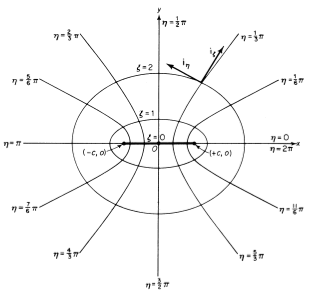
\includegraphics{./Imagenes/Sistema_02_Eliptico_Cilindrico.png}
    \caption{Coordenadas elípticas cilíndricas.}
    \label{fig:figura_coordenadas_elipticas}
\end{figure}
Considerando la figura (\ref{fig:figura_coordenadas_elipticas}) es claro que si acotamos las \emph{coordenadas elípticas} $(\xi, \eta)$ a los rangos
\begin{equation}
    0 \leq \xi < \infty, \hspace{1cm} 0 \leq \eta < 2 \: \pi
    \label{eq:ecuacion_A_11_03}
\end{equation}
cada punto $(x, y)$ en un plano $z = \mbox{ constante}$ se representa al menos una vez y, con la excepción de los puntos $(-c < x < c, y = 0)$ (para los cuales $\eta$ está evaluada dos veces).
\par
Eliminando $\eta$ de la ec. (\ref{eq:ecuacion_A_11_02}) se obtiene
\begin{equation}
    \dfrac{x^{2}}{c^{2} \: \cosh^{2} \xi} + \dfrac{y^{2}}{c^{2} \: \sinh^{2} \xi} = 1
    \label{eq:ecuacion_A_11_04} 
\end{equation}
Por lo tanto, la familia de curvas en el plano $x-y$ caracterizadas por el parámetro constante $\xi$, son elipses que tienen sus centros en el origen. 

Además, ya que $\cosh \xi > \sinh \xi \geq 0$ los semiejes mayor y menor, $a_{0}$ y $b_{0}$ respectivamente, para una elipse típica $\xi = \xi_{0} = \mbox{ constante}$, son
\begin{equation}
    a_{0} = c \: \cosh \xi_{0}, \hspace{1cm} b_{0} = c \: \sinh \xi_{0}
    \label{eq:ecuacion_A_11_05}
\end{equation}
Éstas se encuentran a lo largo de los ejes $x$ e $y$, respectivamente. De la ec. (\ref{eq:ecuacion_A_11_05}), se tiene que
\begin{equation}
    a_{0}^{2} + b_{0}^{2} =  c^{2}
    \label{eq:ecuacion_A_11_16}
\end{equation}
de lo cual se deduce que la familia de las elipses son confocales, es decir, cada elipse de la familia tiene los mismos focos. Los dos focos están en el eje $x$, en los puntos $(x = \pm c, y = 0)$, que corresponden a los valores $(\xi=0, \eta = 0)$ y $(\xi = 0, \eta = \pi)$, respectivamente. Al eliminar $c$ de la eq. (\ref{eq:ecuacion_A_11_05}) finalmente obtenemos
\begin{equation}
    \xi_{0} = \dfrac{1}{2} \: \ln \dfrac{a_{0} + b_{0}}{a_{0} - b_{0}}
    \label{eq:ecuacion_A_11_07}
\end{equation}
esta ecuación expresa el parámetro $xi_{0}$ en términos de las longitudes de los semiejes.

La excentricidad de la elipse $\xi = \xi_{0} = \mbox{ constante}$ es
\begin{equation}
    e_{0} = \left[ 1 - \left(\dfrac{b_{0}}{a_{0}} \right)^{2} \right]^{1/2} = \sech \xi_{0}
    \label{eq:ecuacion_A_11_08}
\end{equation}
La ec.(\ref{eq:ecuacion_A_11_02}) muestra que cuando $\xi_{0} = 0$ la elipse es degenerada y corresponde a ese segmento del eje $x$ que se encuentra entre los dos focos,  es decir, la línea se compone de los puntos $(-c \leq x \leq c, y = 0)$. Mientras $\xi_{0} \to \infty$, la elipse se aproxima a un círculo de radio infinito.
\end{document}